\documentclass{exam}
\usepackage[utf8]{inputenc}
\usepackage[margin=1in]{geometry}
\usepackage{amsmath}
\usepackage{siunitx}
\usepackage{graphicx}
\usepackage{multicol}
\usepackage{etoolbox}
\usepackage{intcalc}
\usepackage{framed}
\usepackage{tabu}
\usepackage{tabularx}
\newcommand{\match}[2]{
	\begin{tabularx}{\textwidth}{r X}
		\fillin[#1][0.5 in] & #2
	\end{tabularx}}
\newcounter{wbcount}
\newcommand{\wbelem}[1]{\stepcounter{wbcount}
	\textbf{\Alph{wbcount}} & {#1}
	\ifnumequal{0}{\intcalcMod{\value{wbcount}}{\wbcolsize}}
		{\\}
		{&}
}
\newenvironment{wordbank}[1]{
	\renewcommand*{\arraystretch}{1.5} \def\wbcolsize{#1}
	\begin{center} \begin{framed}
	\begin{tabu} to \textwidth {*{#1}{X[1,l] X[5,l]}}
	}
	{\end{tabu} \end{framed} \end{center}
}
\setlength\answerclearance{3 pt}

\usepackage{xcolor}
\newcommand{\choiceblank}[1]{
	\ifprintanswers \underline{\ \ #1\ \ }
	\else \underline{\hspace{0.40 in}}
	\fi
	\vspace{0.05 in}
}
\newcommand{\fixcolspacing}{\vspace{0pt plus 1filll}\mbox{}}
\renewcommand{\solutiontitle}{}
\unframedsolutions
\SolutionEmphasis{\color{violet}}

\usepackage{physics}
\usepackage{hyperref}

\pagestyle{head}
\header{Class}{Exam title - Page \thepage}{Student ID:\kern .5 in}
\headrule

\begin{document}
\begin{coverpages}
	\begin{center}
		\vspace{0.05 in}
		\par\noindent\textbf{\large  Subtitle}
		\vspace{0.05 in}
		\vspace{0.10 in}
		\par\noindent\textbf{\Huge   Title}
		\vspace{0.5 in}
		\par\noindent
		\vspace{0.05 in}
		\par\noindent
				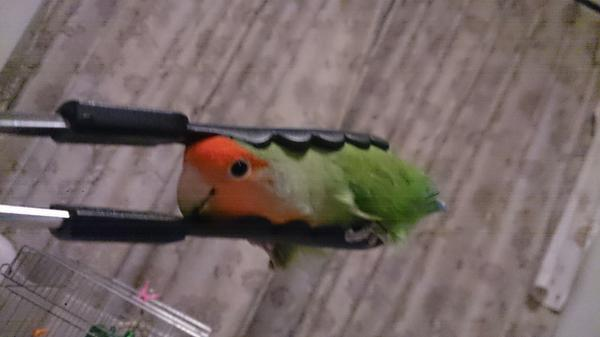
\includegraphics[width=.7\textwidth]{images/tong.jpg}
		\vspace{0.05 in}
		\vspace{0.5 in}
		\vspace{0.10 in}
		\vspace{0.15 in}
		\par
		\def\arraystretch{2}\tabcolsep=3pt
		\begin{tabular}{r r}
			\textbf{Student Name:} & \makebox[4in]{\hrulefill} \\
			\textbf{Date:} & \makebox[4in]{\hrulefill} \\
			\textbf{Any other info:} & \makebox[4in]{\hrulefill} \\
		\end{tabular}
		\vspace{0.15 in}
	\end{center}
		\vspace{0.10 in}
	\par\noindent The order of modules within sections roughly corresponds to the order in which they're generated as tex. For example, putting the subtitle module before the title module results in the subtitle being rendered above.
	\par Throughout the exam, you can use the following bangs: gap (which inserts vertical space), img (which inserts an image with the given filename and renders it at the given width), and newpage (self explanatory). Other bangs are specific to certain modules.
		\vspace{0.10 in}
	\begin{center}
		\vspace{0.05 in}
		\par
		\def\arraystretch{2}\tabcolsep=3pt
		\begin{tabular}{r r}
			\textbf{{Written by:}}
			 & \textbf{ Dhruva ``deorge'' Karkada}, \textit{ dkarkada@gmail.com} \\
		\end{tabular}
		\vspace{0.05 in}
	\end{center}
\end{coverpages}

\newpage
\par\noindent \textbf{\large  Matching}
	\par\noindent  2 points each. Each choice will be used; some more than once.
\begin{wordbank}{3}
	\wbelem{Answer 1}
	\wbelem{Answer 2}
	\wbelem{Answer 3}
	\wbelem{Answer 4}
	\wbelem{Answer 5}
	\wbelem{Answer 6}
	\wbelem{Answers}
	\wbelem{Extra ans}
	\wbelem{Otherwise}
	\wbelem{Questions}
	\wbelem{The option}
	\wbelem{Unless}
\end{wordbank}
\begin{questions}
\setcounter{question}{0}
	\question\match{F}{This is question 6}
	\question\match{A}{This is question 1}
	\question\match{L}{You include `noshuffle' as an option}
	\question\match{C}{This is question 3}
	\question\match{E}{This is question 5}
	\question\match{G}{are sorted alphabetically, while}
	\question\match{D}{This is question 4}
	\question\match{G}{which are used more than once will only appear once in the wordbox}
	\question\match{J}{Will automatically shuffle}
	\question\match{K}{ans=sheet will create a separate answer sheet at the end}
	\question\match{B}{This is question 2}
	\question\match{I}{No dedicated answer sheet will be created}
\end{questions}

\newpage
\par\noindent \textbf{\large  True/false questions}
\begin{questions}
\setcounter{question}{13}
	\question\match{T}{A new section will create a page break.}
	\question\match{T}{The true/false section is just like the matching, except no word bank is created}
	\question\match{T}{And instead of lettering the choices in the word bank, the answer is either `T' or 'F'}
	\question\match{F}{Mars is blue}
	\question\match{F}{America was founded in 1634}
	\question\match{T}{This \LaTeX\ tool is really cool and useful}
\end{questions}

\newpage
\par\noindent \textbf{\large  The title is Multiple Choice}
\setlength{\columnsep}{0.40 in}
\begin{multicols*}{2}
\renewcommand{\choiceshook}{\setlength{\leftmargin}{0.40 in}}
\renewcommand{\questionshook}{\setlength{\leftmargin}{0.0 in}}
\begin{questions}
\setcounter{question}{19}
	\question[2] New sections automatically
	\begin{choices}
		\choice z
		\choice z
		\CorrectChoice Create a pagebreak
	\end{choices}
	\question[2] Multiple choice questions
	\begin{choices}
		\choice z
		\choice z
		\choice z
		\CorrectChoice automatically have answers shuffled
	\end{choices}
	\question[2] Unless you mark the correct answer
	\begin{choices}
		\CorrectChoice with this symbol at the end:
		\choice Then the answer choice order
		\choice will be
		\choice preserved
	\end{choices}
	\question[2] For shuffled questions, put the
	\begin{choices}
		\CorrectChoice correct answer choice first,
		\choice z
		\choice followed by the bogus answers
	\end{choices}
	\question[2] The spacing of MC questions depends
	\begin{choices}
		\choice on the available space on the page
		\CorrectChoice which depends on how much instructions you wrote.
	\end{choices}
	\question[2] So do me a favor and estimate the height taken up by the
	\begin{choices}
		\choice title and instructions
		\CorrectChoice measured in units of pt
		\choice and include that as the option ``intro-height''
		\choice z
		\choice z
		\choice z
	\end{choices}
	\question[2] Better to overestimate than underestimate
	\begin{choices}
		\CorrectChoice or else you might get some funky formatting
		\choice z
		\choice z
	\end{choices}
	\vfill\null\columnbreak
	\question[2] The option ``twocolumn'' does what you think it does
	\begin{choices}
		\CorrectChoice z
		\CorrectChoice z
		\CorrectChoice z
	\end{choices}
	\question[2] The qworth option for MC and matching modules will print the pre-determined point-value
	\begin{choices}
		\CorrectChoice for all questions.
		\choice To print point values for FRQ, see next section
	\end{choices}
\end{questions}
\end{multicols*}
\renewcommand{\choiceshook}{}
\renewcommand{\questionshook}{}

\newpage
\par\noindent \textbf{\large  Free Response}
	\par\noindent  Write legibly
\begin{questions}
	\setcounter{question}{28}
	\question A question can have parts and subparts
	\begin{parts}
		\part Here is a part
		\part Here is another part
		\begin{subparts}
			\subpart Its first subpart
			\subpart Next subpart
		\end{subparts}
		\part Last part
	\end{parts}
	\question 
	\begin{parts}
		\part This question has no high-level question
		\part It only shows these two question parts
	\end{parts}
	\question You can put math here: $y=mx+b$ or alternatively \[i\hbar \frac{\partial \Psi}{\partial t} = -\frac{\hbar^2}{2m}\frac{\partial^2 \Psi}{\partial x^2} + V \Psi\] if you like this better.
	\question You can include commands from packages imported in the header. These come from the physics package: $\laplacian\div\grad\dv{x}$
	\question Quotation ``marks'' and \% symbols are preserved
	\question[3]  Indicate point values by preceding questions with curly bracketed numbers
	\begin{parts}
		\part question1
		\part question2
	\end{parts}
	\question You can also directly put some \LaTeX\ commands in here
		\newpage
\end{questions}
	\par\noindent \noindent\textbf{sss}
	\par \par\noindent Lorem ipsum blah blah
\\ [.2 in]
\par\noindent If you want to insert your own \LaTeX\ for whatever reason, you can do it here.
\par
\begin{itemize}
	\item item 1
	\item item 2
\end{itemize}
\begin{questions}
	\setcounter{question}{35}
	\question Back to some sweet
	\begin{parts}
		\part free
			\begin{solution}[20 pt]
			 free
			\end{solution}
		\part response
			\begin{solution}[20 pt]
			 response
			\end{solution}
		\part questions!
			\begin{solution}[20 pt]
			 questions
			\end{solution}
	\end{parts}
	\question By default, no answer sheet is generated at the end of the exam. You must use the ans option to specify if you want an answer sheet for a given question module
		\begin{solution}[36 pt]
		 ok
		\end{solution}
	\question But of course, every question module shows up in the answer key
		\begin{solution}[36 pt]
		 of course
		\end{solution}
\end{questions}
\begin{center}
\def\arraystretch{1.25}
\begin{tabular}{|c|c|}
\hline
	\textbf{Age} & \textbf{Height}\\
	\hline
	11 & 5'2"\\
	13 & 5'3"\\
	14 & 5'6"\\
	16 & 5'8"\\
	18 & 5'9"\\
\hline
\end{tabular}
\end{center}
\newpage
\section*{Answer Sheet}
	\raggedcolumns
	\begin{multicols}{5}
	\begin{enumerate}
	\setcounter{enumi}{19}
	\item \choiceblank{C}
	\item \choiceblank{D}
	\item \choiceblank{A}
	\item \choiceblank{A}
	\item \choiceblank{B}
	\item \choiceblank{B}
	\item \choiceblank{A}
	\item \choiceblank{A}
	\item \choiceblank{A}
	\end{enumerate}
	\fixcolspacing
	\end{multicols}
	\begin{questions}
	\setcounter{question}{28}
	\question
		\begin{parts}
		\part
			\ \vspace{16 pt}
		\part
			\begin{subparts}
			\subpart
				\ \vspace{16 pt}
			\subpart
				\ \vspace{16 pt}
			\end{subparts}
		\part
			\ \vspace{16 pt}
		\end{parts}
	\question
		\begin{parts}
		\part
			\ \vspace{16 pt}
		\part
			\ \vspace{16 pt}
		\end{parts}
	\question
		\ \vspace{16 pt}
	\question
		\ \vspace{16 pt}
	\question
		\ \vspace{16 pt}
	\question
		\begin{parts}
		\part
			\ \vspace{4 pt}
		\part
			\ \vspace{80 pt}
		\end{parts}
	\question
		\ \vspace{16 pt}
	\end{questions}
\end{document}